\chapter{Line Rendering}

As a sketching application, it is important for curves to be rendered with high quality.
While graphics hardware has support for line rendering, it's implementation is only suitable for line segments, with significant issues when trying to render curves.
In this chapter, we discuss the system this project implements for curve rendering.

\section{Problems With Available Line Renderers}
OpenGL has support for a variety of line primitives: lines, line strips, and lines with adjacency data.
However, these primitives are not suited for rendering curves at high quality.
This is because of the method OpenGL uses to render line segments: as a rectangle between the two segment points.
While this method is suited for common uses of lines in 3D applications, for example wire frames, it does not extend to curve rendering because of the gaps that appear between segments.
It is reasonable to think that if we use a curve that is subdivided to a fine enough degree, then the holes will be so small that they would not be visible.
However, in practice, even finely subdivided lines have visible holes around any curve.

\begin{figure}
	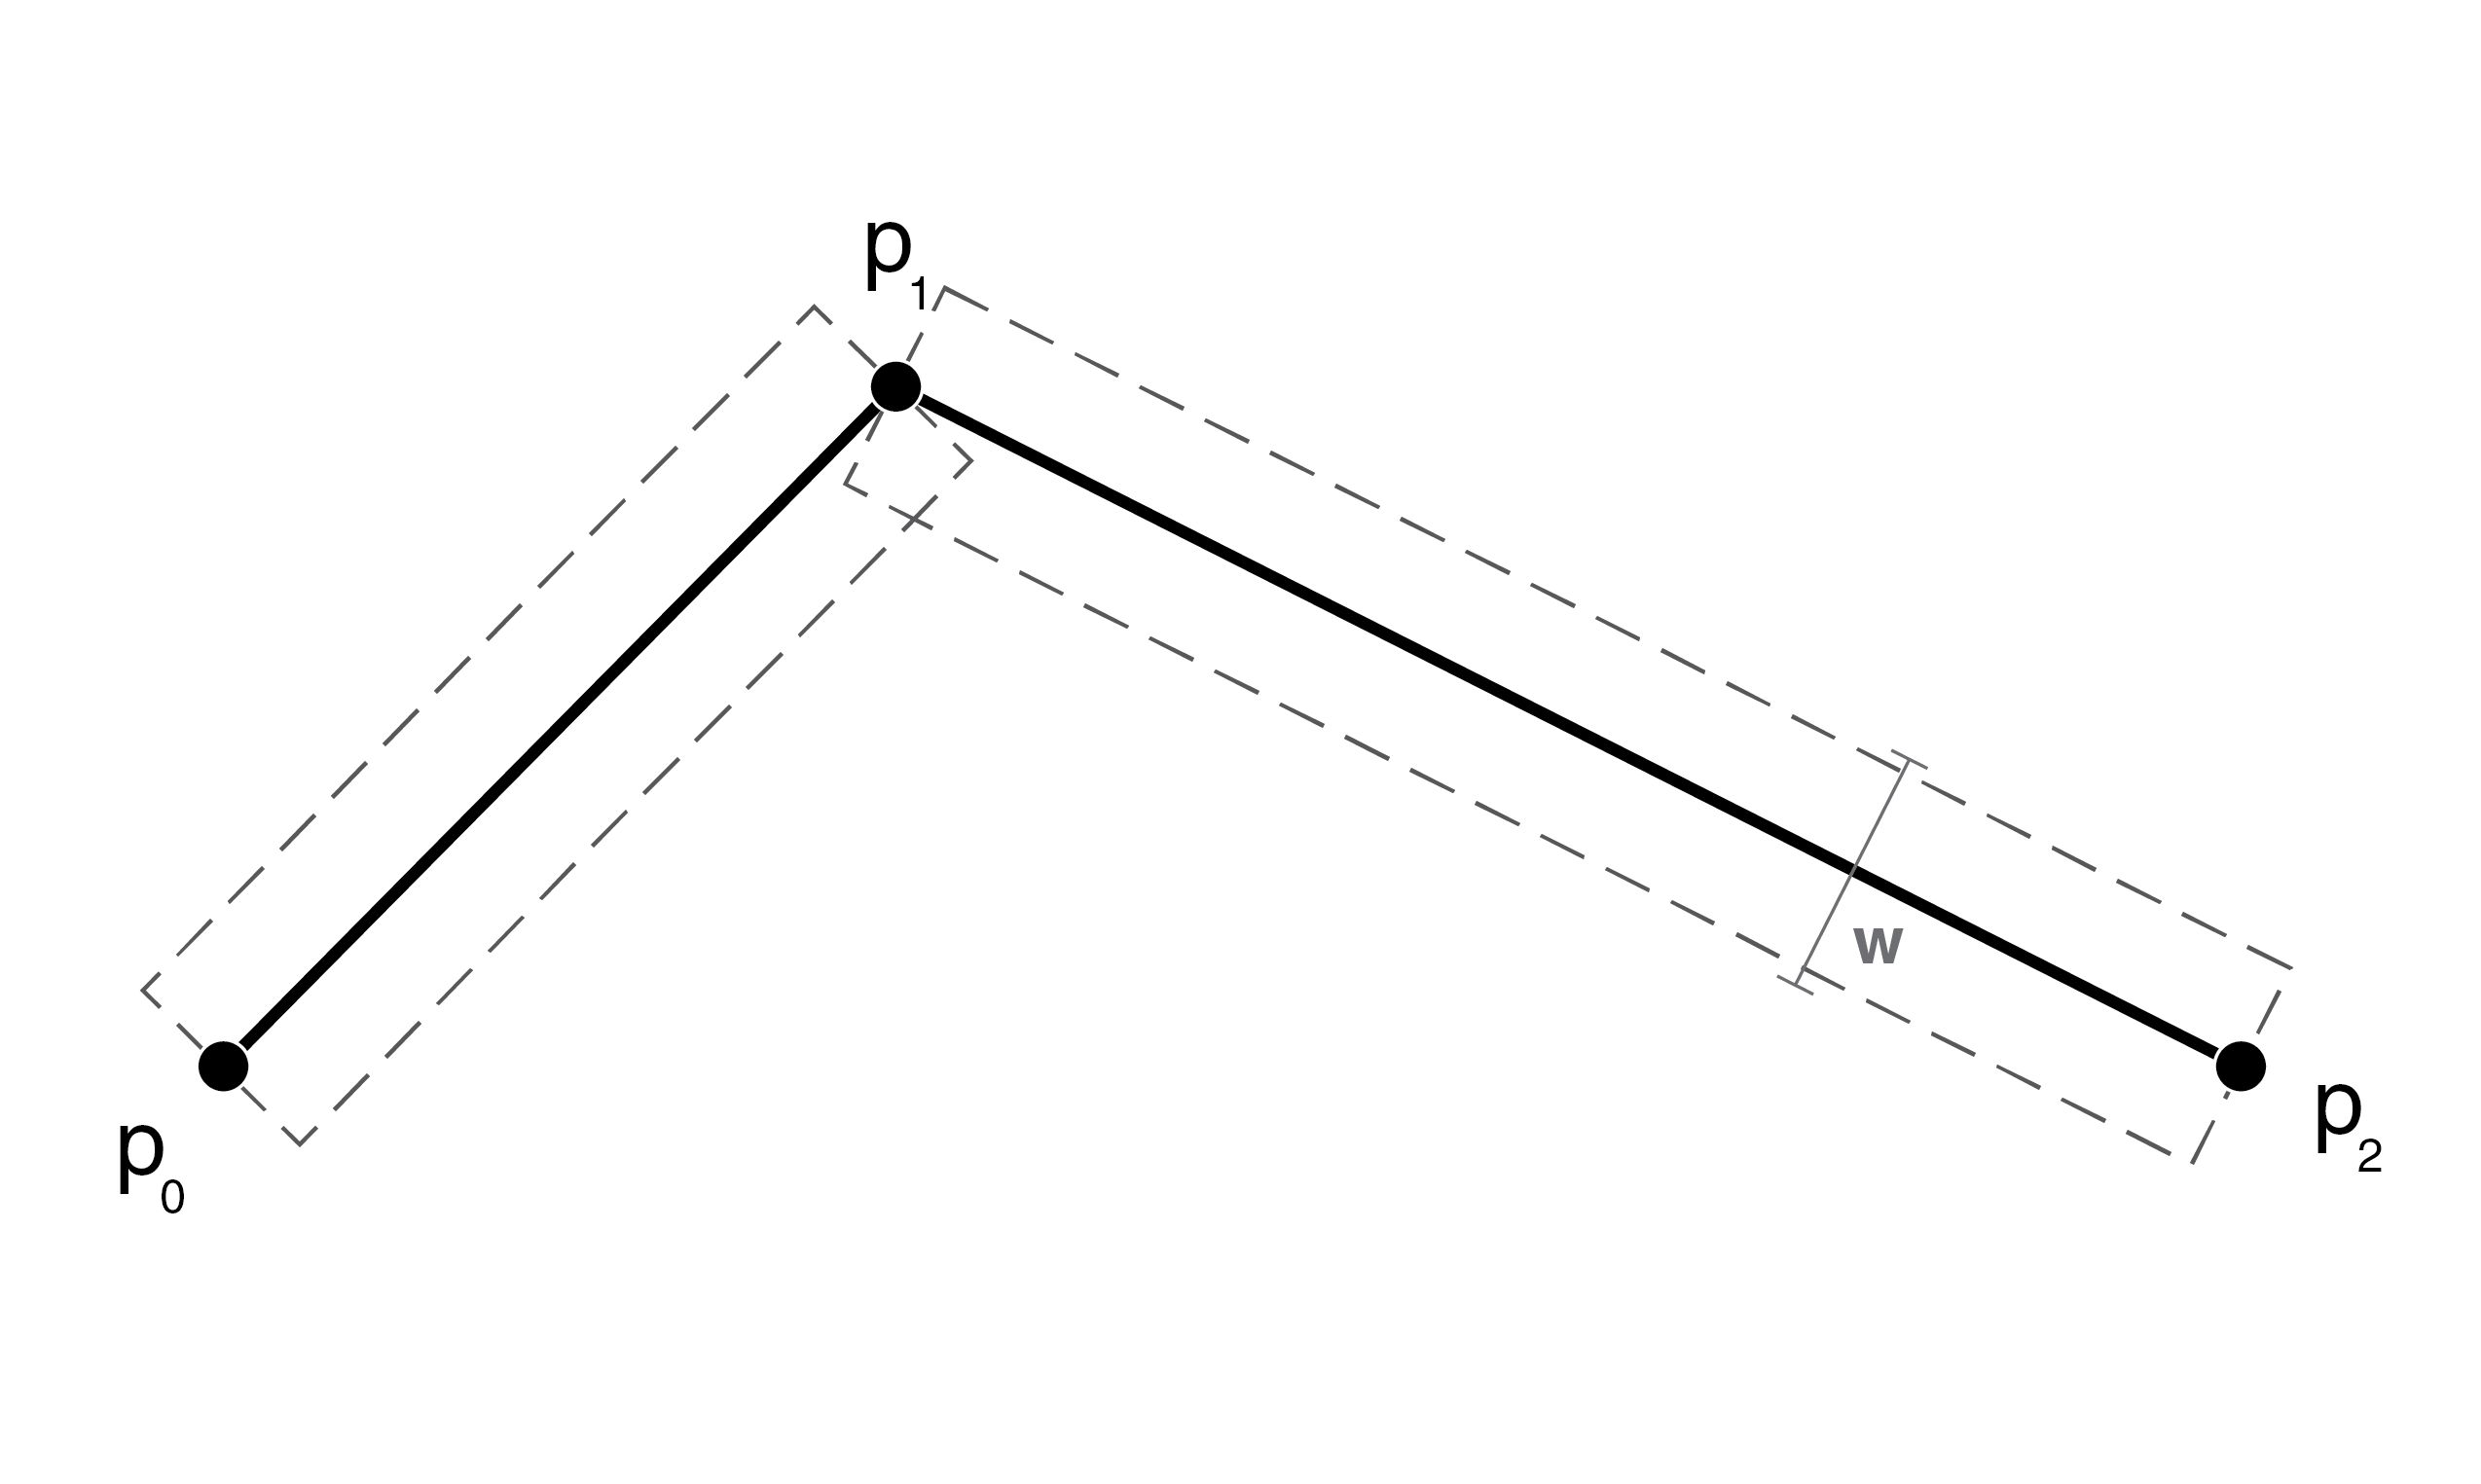
\includegraphics[width=\textwidth]{linesegment2.png}
	\caption{Two line segments connected together, as per default GL\_LINES implementation. Note the gap from no join.}
\end{figure}

To correct the holes, this project implements a custom line renderer that constructs a triangle mesh from the line definition.
Constructing a mesh for the line allow allows for implementation of a wide variety of stroke types, including strokes with various end caps or variable width based on stroke direction. 

Additionally, OpenGL lines have inconsistent support for anti-aliasing across all hardware.
By switching to a triangle mesh, we leverage the native anti-aliasing support for triangles without worrying about consistency.
As we can see in the above image, without anti-aliasing rendered lines appear jagged and poor quality.
In order for our system to be appealing as a drafting table replacement, our system needs to render the highest quality lines possible.

\begin{figure}
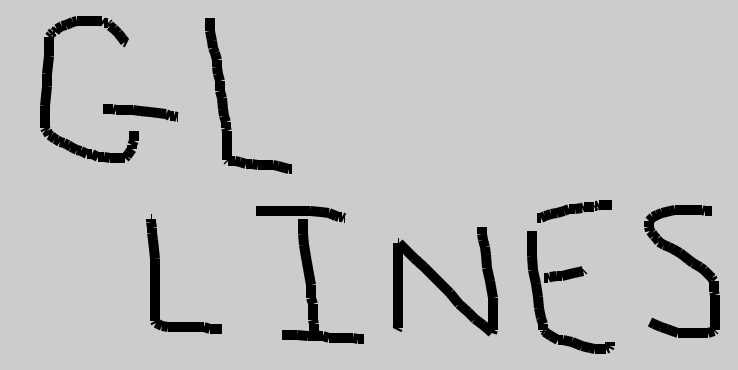
\includegraphics[width=\linewidth]{gllines}
\caption{An example of the flaws of native line rendering in OpenGL using GL\_LINES.}
\end{figure}

\pagebreak
\section{Creating Joins From the Line Definition}

\begin{table}
\begin{center}
\begin{tabular}{|c|l|}
\hline
\textbf{Symbol} & \textbf{Description} \\ \hline
$p_n$			& Ordered point on line in the range $[0,2]$ \\
$n_{xy}$		& The normal to the line segment $(p_x, p_y)$ \\	
$t_x$			& Vector from $p_1$ along $n_{x1}$ with length $line\_width/2$ \\
\hline
\end{tabular}
\caption{Section Variables} \label{tab:linevariables}
\end{center}
\end{table}

In order to improve the appearance of our curves relative to the native OpenGL implementation, we will need to compute joins between each of our line segments.
For this project, we implement three types of joins: miter, bevel, and round.
Miter and bevel joins are used in conjunction with each other, while round joins are used alone.

A round join is formed by rounding out the gap such that a smooth curve is created. 
It is calculated by forming a circle whose center is located at $p_1$, with a radius of $line\_width/2$. 
The total angle that needs to be filled can be calculated by $t_0 \cdot t_2$, and can be filled by rotating either $t_0$ or $t_2$ about $p_1$.

Miter joins are formed by extending the lines in the line geometry parallel to the original segment.
The join is formed where these extended lines intersect, as can be seen in Figure 1.5.
To calculate this, we take the line segments defined by $(p_0 + t_0, p_1 + t_0)$ and $(p_2 + t_2, p_1 + t_2)$ and compute their intersection. We call the vector from this intersection to $p_1$ $v$.
We can then compute a polygon between $p_1$, $p_1 + t_0$, $p_1 + t_2$, and $p_1 + v$, which creates the miter join. 

\begin{figure}
	\begin{center}
		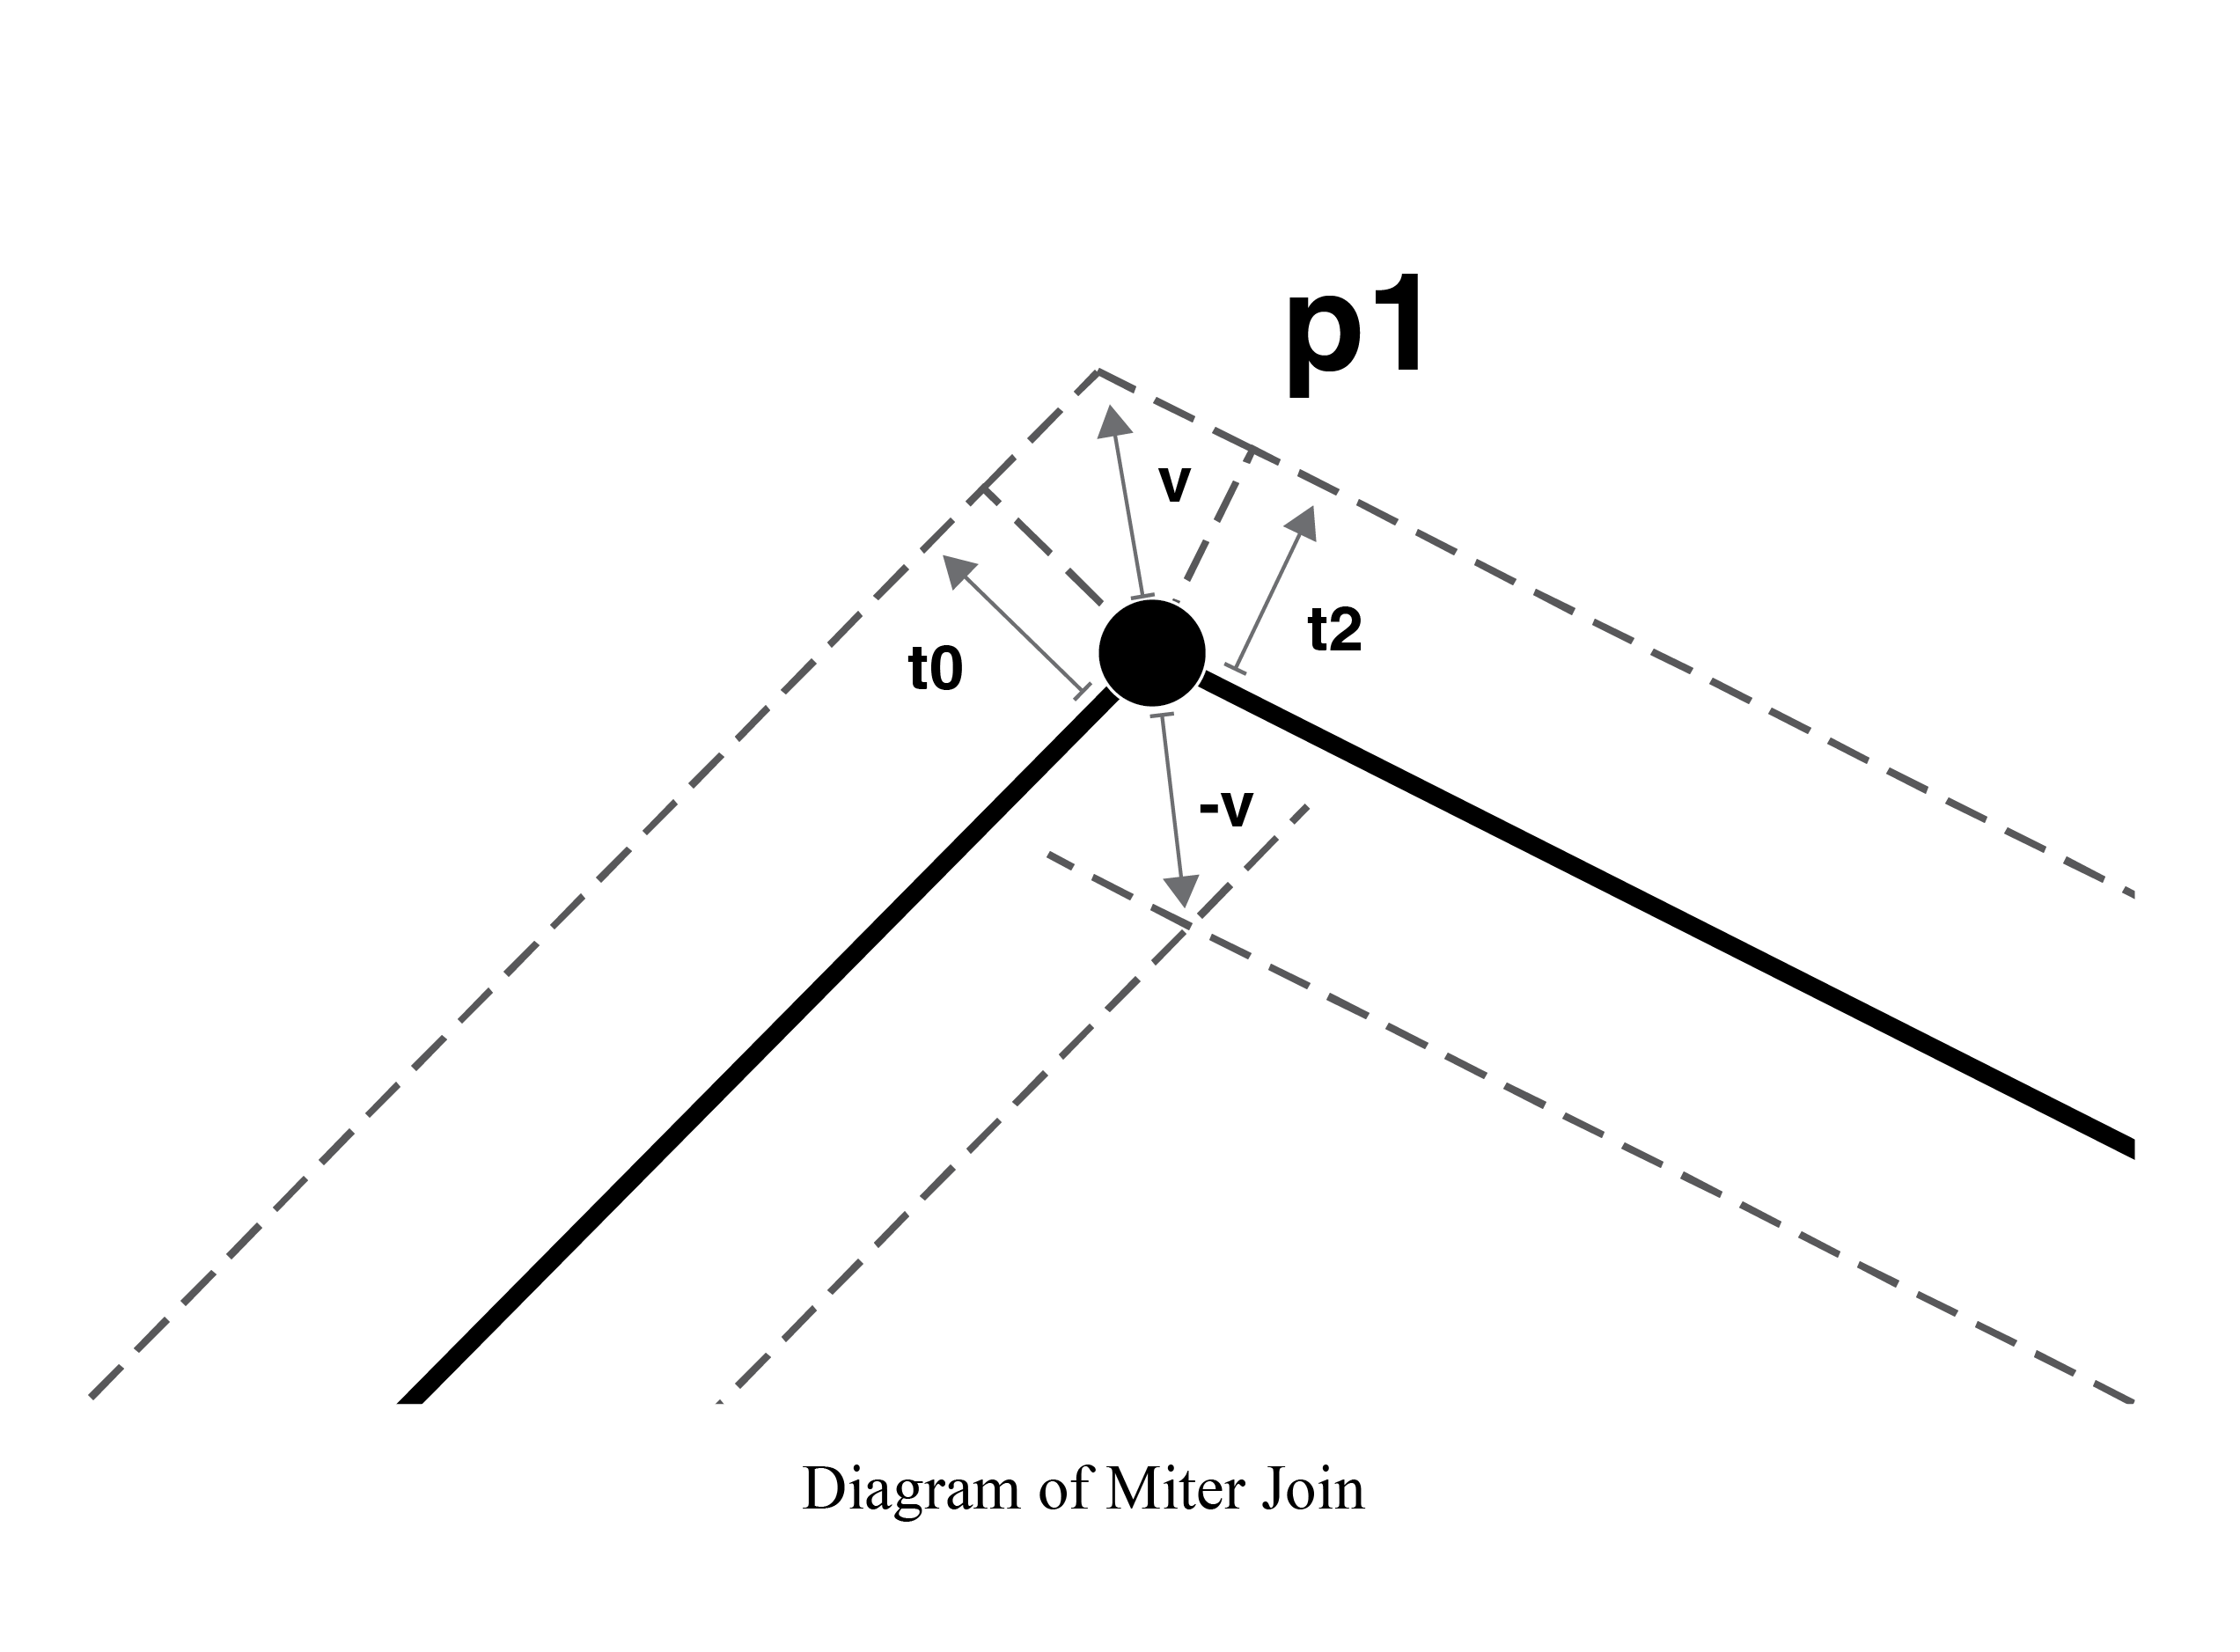
\includegraphics[width=0.7\textwidth]{miter.png}
		\caption{Diagram of a miter join with parameter labels}
	\end{center}
\end{figure}

\begin{figure}
	\begin{center}
		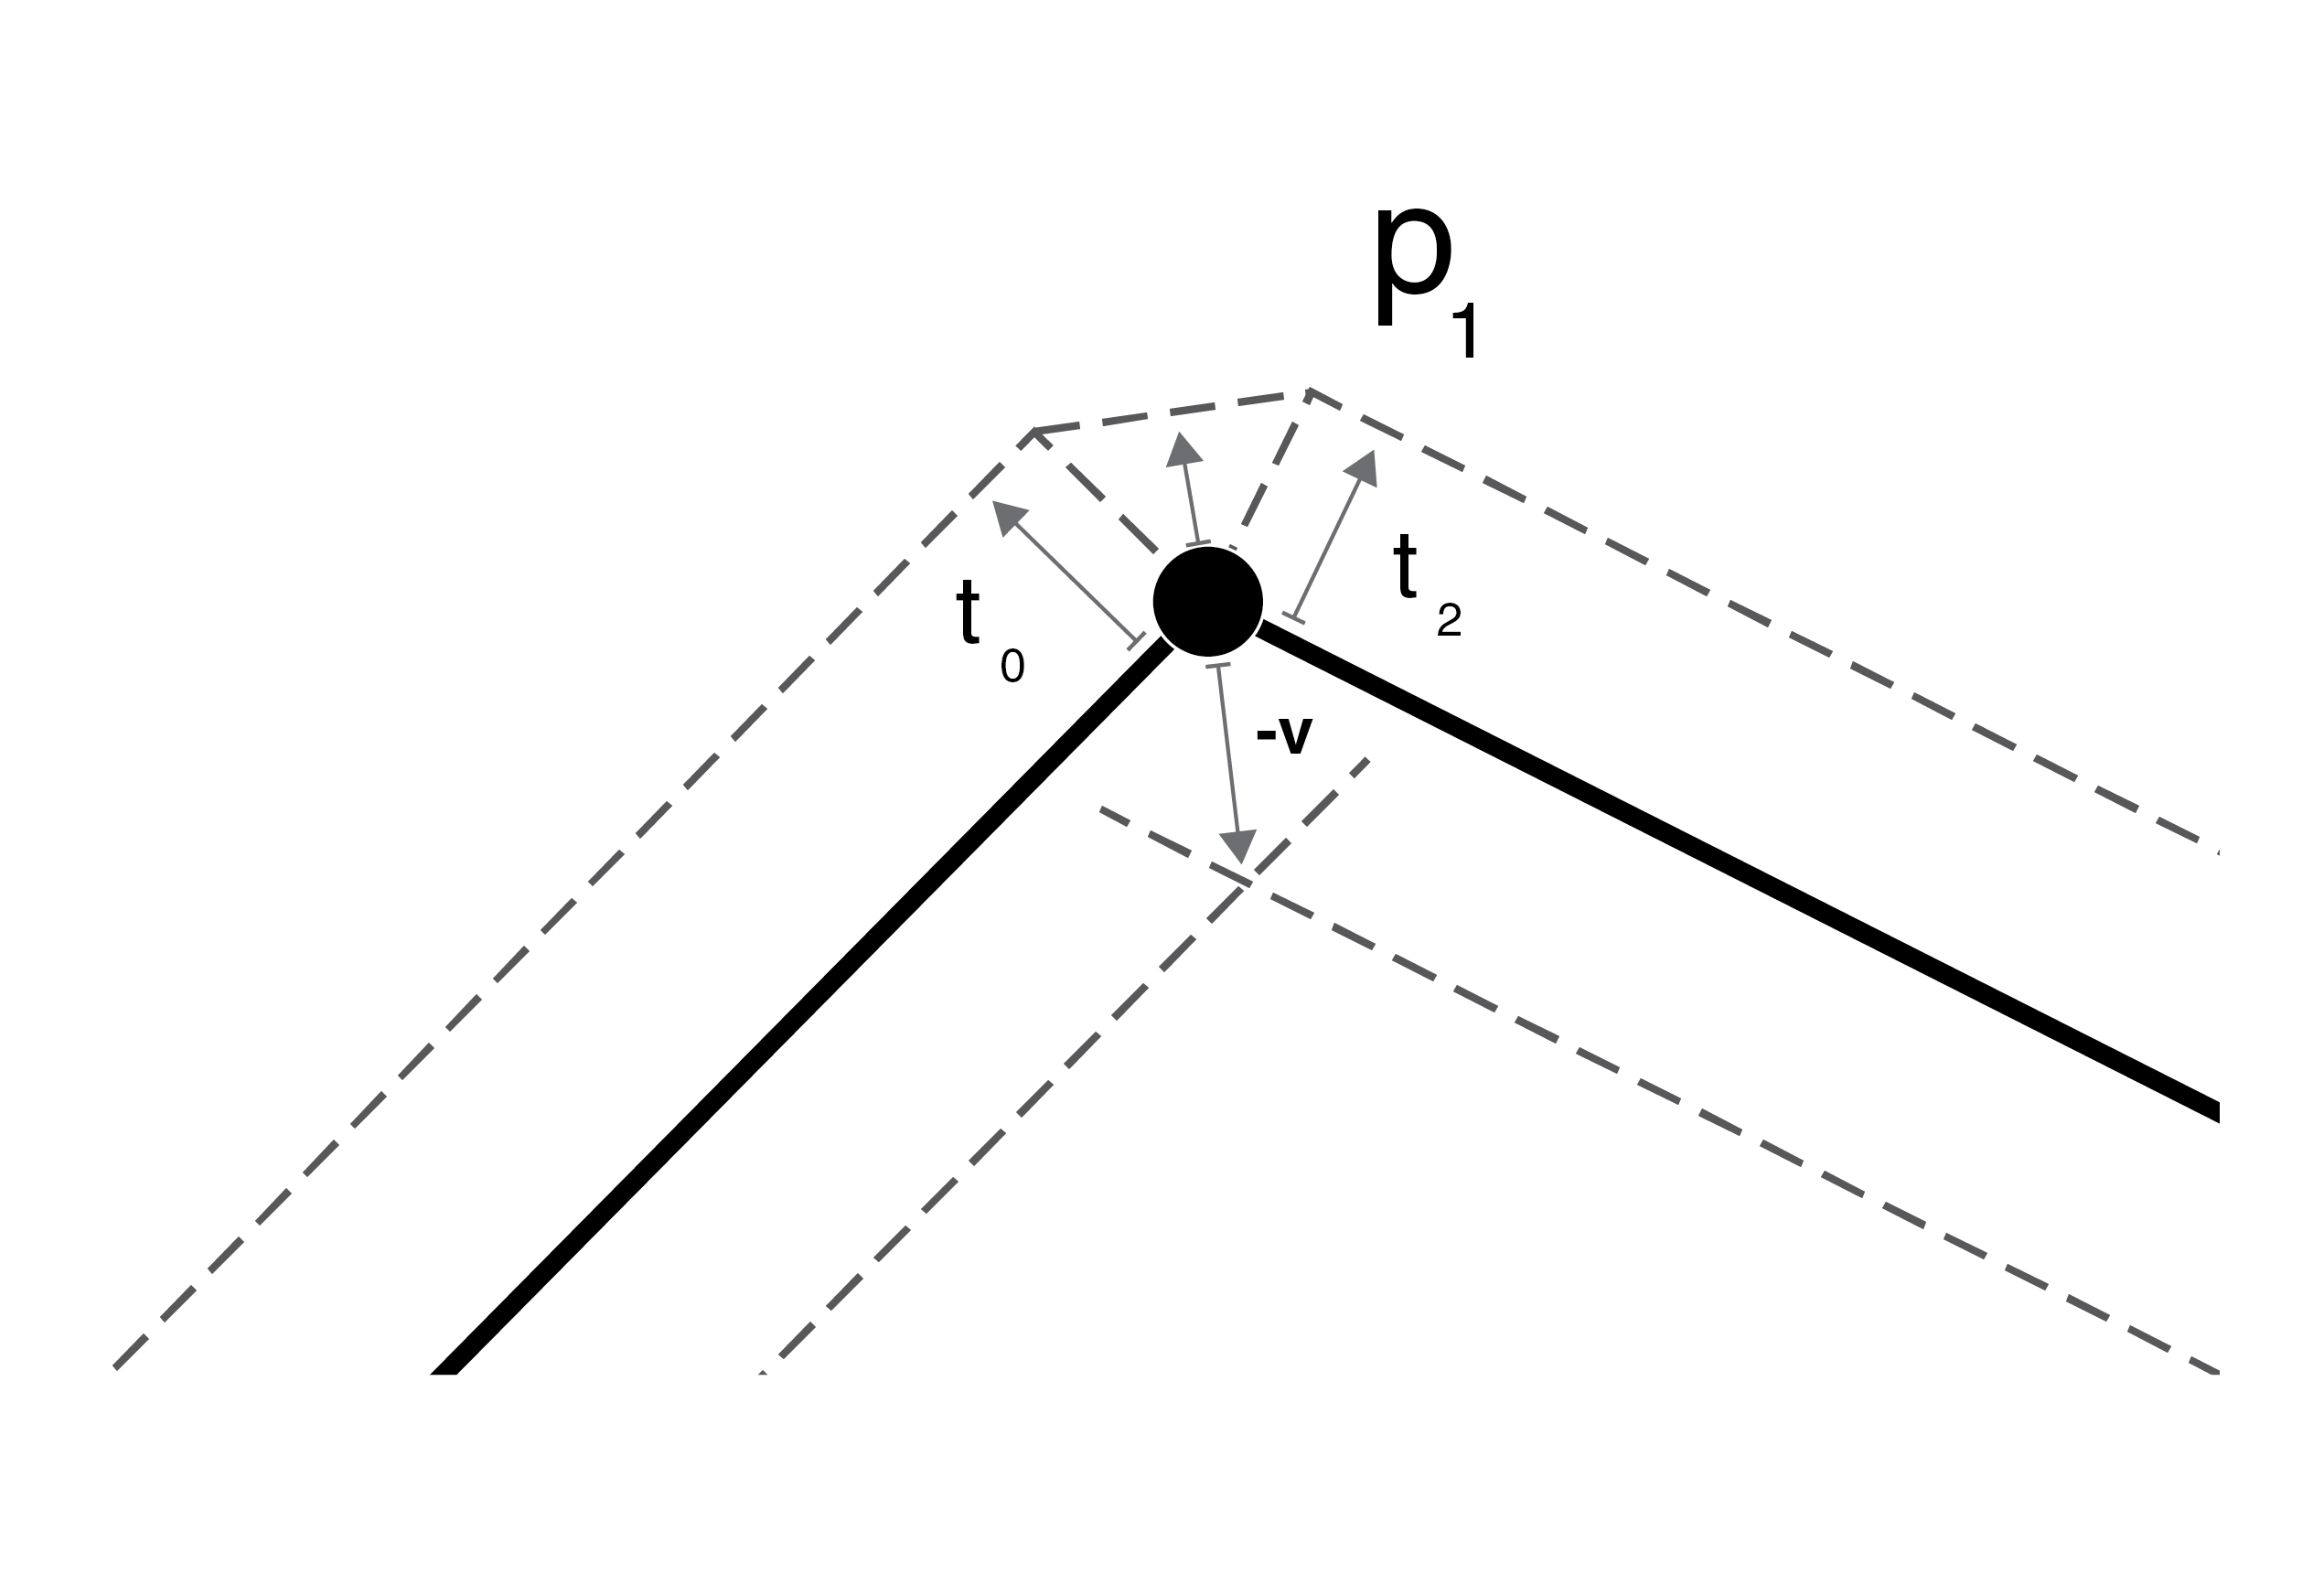
\includegraphics[width=0.7\textwidth]{bevel.png}
		\caption{Diagram of a bevel join with parameter labels}
	\end{center}
\end{figure}

\begin{figure}
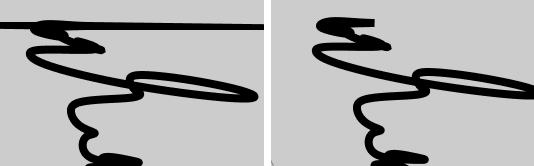
\includegraphics[width=\textwidth]{joinartifact.png}
\caption{Left: An example of a miter join artifact from a sharp curve. Right: Artifact post-correction.}
\end{figure}

Miter joins have the particular issue that artifacts can arise from exceptionally sharp points in the line segments.
We detect these cases by checking to see if $v$ is larger than a certain length.
If so, we use a bevel join instead.
The bevel join is formed by simply creating a triangle between $p_1$, $p_1 + t_0$, and $p_1 + t_2$.

\pagebreak
\section{Implementation}

Actually creating this geometry can get very expensive, especially as more and more lines are drawn. 
A simple polygonalization for a robust miter and bevel join implementation can create as many as six polygons for each pair of points on the curve.
This does not take into account round joins, as smooth circle approximations require a large number of polygons.
Combine this with spline subdivision, and we run the risk of running into bandwith problems when transferring polygon data between the GPU and the CPU for very large strokes.
To solve for this, we implement these algorithms in a geometry shader using a line adjacency data structure input.
In order to reduce the number of branch operations, we polygonalize each line segment in halves, taking care of the join calculation for each side separately.
An example of a polygonalized line segment can be seen in Figure 1.8.

\begin{figure}
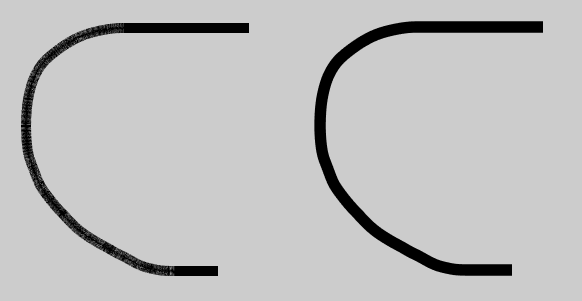
\includegraphics{linerendering}
\caption{Left: A curve using default GL\_LINES. Right: Implemented system}
\end{figure}

\begin{figure}
	\begin{center}
		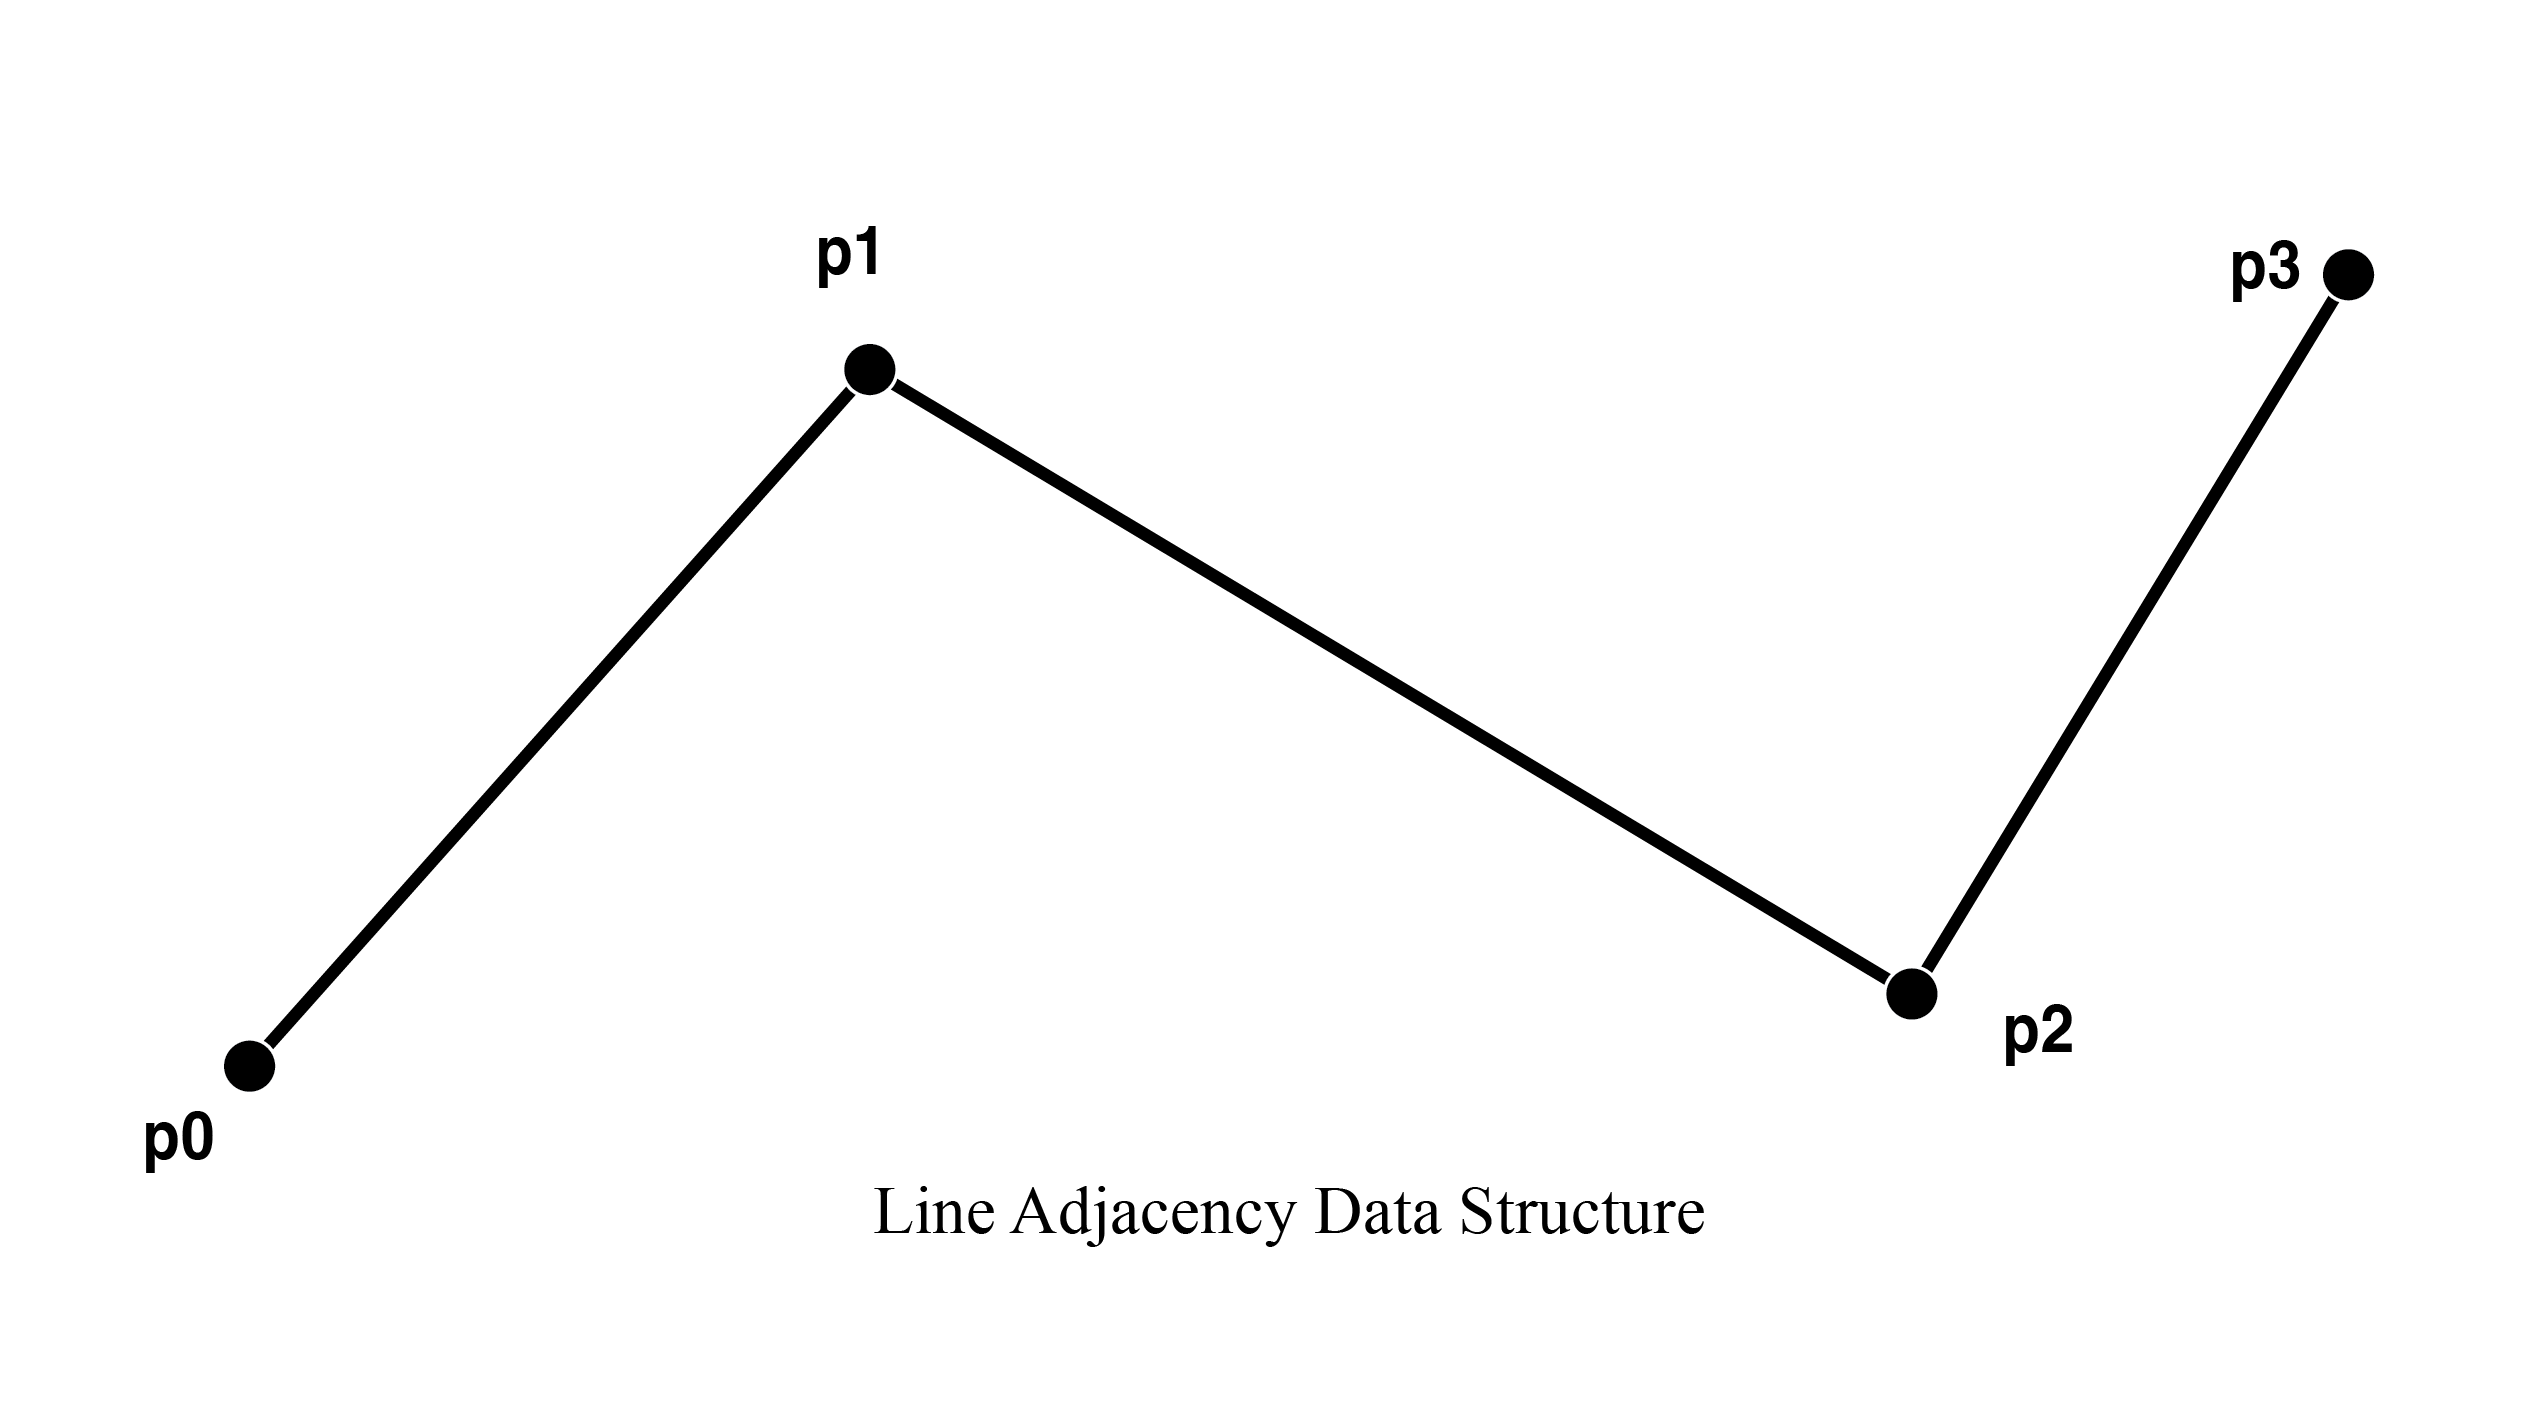
\includegraphics[width=\textwidth]{lineadjacency.png}
	\end{center}
	\caption{The line adjacency data structure. Each instance of the geometry shader polygonalizes the line segment (p1, p2)}
\end{figure}
\begin{figure}
	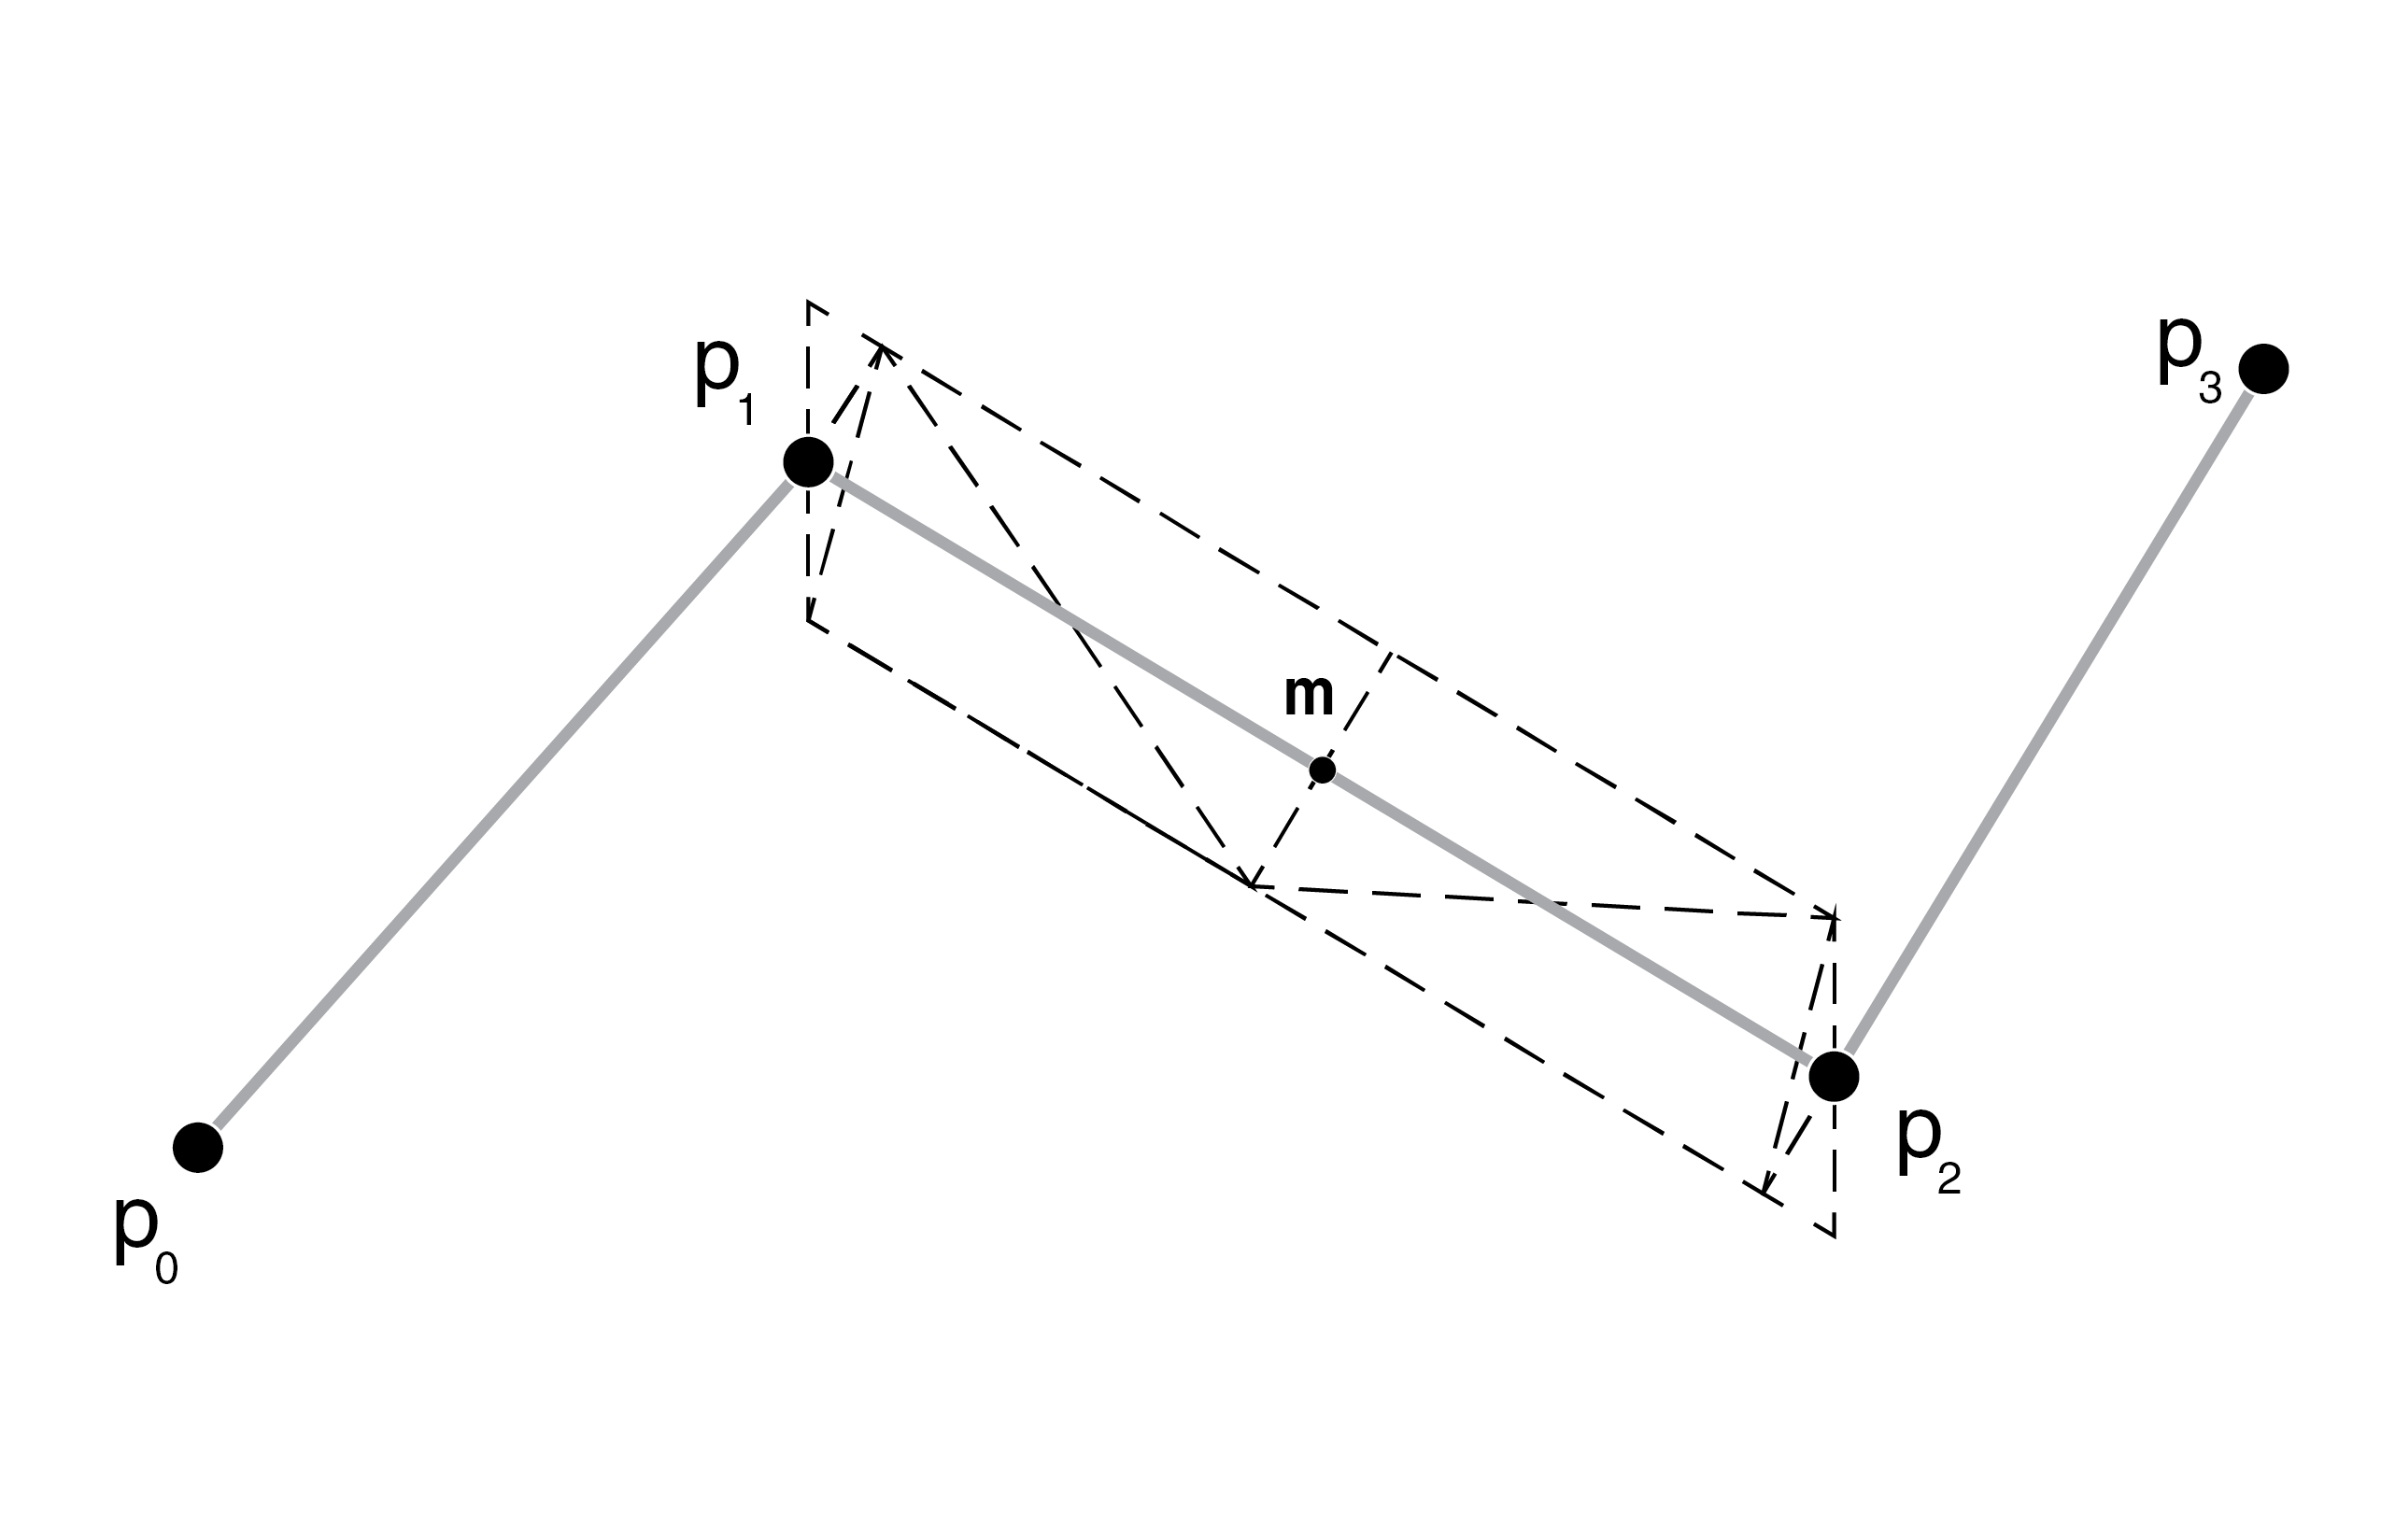
\includegraphics[width=\textwidth]{linepolyex.png}
	\caption{Example polygonization of a line with miter joins.}
\end{figure}



The system can now display polygonalized, three dimensional lines and does so efficiently.
However, we still need to decide how we are going to expand our lines.
Approaches similar applications have taken include: 
\begin{itemize}
\item Creating the line geometry on the screen and projecting it onto scene objects. With this approach, lines only exist on the plane they are drawn on. Because of this, it is possible to turn the camera and not see strokes the user has already mode. This approach is only suitable for applications where a base geometry is already supplied, and therefore not suitable for early stage design applications. Other shortcomings include the requirement of a large number of ray cast operations for each line created, which puts too much work on the CPU for a real time application, as well as the lines created lacking a sense of depth.
\item Creating 3-D geometry from the line definition. This approach makes lines look poor when viewed from the side, as the line form will not have the same shape as originally intended. The approach also requires a high number of polygons.
\end{itemize}

We would like to allow for lines to be viewed from any direction, while still retaining their original line width and quality.
The approach this application takes is to perform all of the calculations from creating line geometry in the distorted image space.
By working in the distorted image space, we can guarantee the geometry is always expanded in the screen's x-y plane.
Since points in the distorted space also contain a z value, our lines will have different widths depending on depth.

\begin{algorithm}[H]
\caption{Line Rendering Algorithm}
\begin{algorithmic}[1]
\For{Line Adjacency data set \{$p_0$, $\cdots$, $p_3$\}}
\State Covert world space line points \{$p_0$, $\cdots$, $p_3$\} to the distorted image space points \{$p_{0s}$, $\cdots$, $p_{3s}$\}
\State Compute normals for each of the line segments $(p_{ns},p_{(n+1)s})$
\State Enforce normals are pointing towards the outer arcs of segment pairs
\State Compute join parameters using image space variables and a defined line width
\State Triangulate for the line segment ($p_1$, $p_2$)
\EndFor
\end{algorithmic}
\end{algorithm}

\begin{figure}
\begin{center}
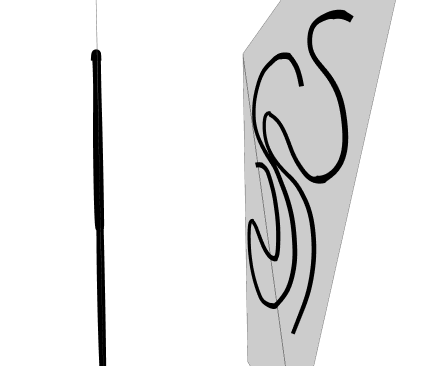
\includegraphics[width=0.5\textwidth]{rotation.png}
\caption{Even when rotating the drawing plane such that it is no longer visible, our lines remain visible.}
\end{center}
\end{figure}

In this chapter we have described a method for creating geometry from a line definition.
We have also described how we create this 2-D geometry such that it is visible from any 3-D direction.
Similar applications create the extra line geometry on the CPU.
By creating our geometry exclusively on the GPU, we minimize the bandwidth needed to transfer data from the CPU to the GPU, allowing extremely detailed curves using our spline calculation.